\chapter{Introduction}
\textcolor{red}{need to fill in}
\section{Formal Definition}
How can we measure the concept of community?  While traditional definitions relied on counting the number of internal and external edges, the modern perspective emphasizes the probability of vertices sharing edges within a subgraph \cite{userguide}. The existence of communities suggests that vertices have stronger interactions with members of their own community compared to other vertices belonging to different communities. As a result, vertices within the same community are more likely to form connections with each other than with vertices outside their community. Therefore, this gives rise to a natural definition of community.
\begin{definition}[Community]
   For a graph $G=(V,E)$, we say $\mathcal{C}\subseteq V$ is a community if for $\forall v\in \mathcal{C}$, we have $\mathbb{P}\left(\{v,u\}\in E\right)>\mathbb{P}\left(\{v,u'\}\in E\right)$ for $\forall u\in \mathcal{C}$ and $u'\in V\setminus \mathcal{C}$.
\end{definition}
\begin{remark}
    In this report, the terms 'community' and 'group' are used interchangeably.
\end{remark}
In order to study the community detection problem, we need some rigorous mathematical framework. There are a variety of effective models, such as \textit{Markove random field} and \textit{factor graph model}. But this report adopts an probabilistic generative models, called \textit{stochastic block model (SBM)}, because it is arguably the most representative one due to its canonicality \cite{Emmanuel2023} \cite{deeplearning}.
\begin{definition}[Stochastic Block Model]
Consider a graph $G=(V, E)$ generated by the Stochastic Block Model $SBM(n, k, \mathcal{P})$, where $n$ is the number of vertices, $k$ denotes the number of communities, and $\mathcal{P}$ is a $k\times k$ probability matrix. Under this model, the graph $G$ possesses a built-in community structure, let $\Omega$ denote the set of communities, then each vertex $v$ is assigned to a community $\sigma_v\in\Omega$, where $\sigma$ is called the planted assignment. For any pair of vertices $u, v \in V$, the probability that there is a connection between $u$ and $v$ is specified by $\mathcal{P}_{\sigma_u, \sigma_v}$, independent of other pairs of vertices. We also define the community sets as $\Omega_i:=\{v\in[n]: \sigma_v=i\}$ for $i\in\Omega$.
\end{definition}
\begin{remark}
    In simple terms, each pair of vertices is connected with probability that only depends on their communities. 
\end{remark}
This report focus on the case where communities have equal size, i.e. $|\Omega_i|=|\Omega_j|$ for $\forall i, j\in\Omega.$. Therefore, we will assume this without specifying it explicitly from now on.\\

We also introduce the symmetric SBM:
\vspace{-2mm}
\begin{definition}[Symmetric SBM]
A symmetric SBM SSBM is a SBM where the $\sigma_v$ are chosen uniformly and for $\forall u, v\in V,$ \begin{equation}
    ~~~~~~~~~~~~~~~~~~~\mathbb{P}\left(\{u,v\}\in E\right) = 
    \begin{cases} 
    p_{\text{in}} & \text{if } \sigma_u = \sigma_v \\
    p_{\text{out}} & \text{if } \sigma_u \neq \sigma_v 
    \end{cases}
\end{equation}
i.e. the probability matrix $\mathcal{P}$ takes the value $p_{in}$ on the diagonal and $p_{out}$ off the diagonal.
\end{definition}
\begin{remark}
    if $p_{in}=p_{out},$ then it reduces to the Erd\H{o}s-R\'{e}nyi random graph.
\end{remark}
In this report, we focus on the symmetric case with $p_{in}>p_{out}$, which is called \textit{homophily} or \textit{assortativity.}\\
Let $c_{in}$ be the expected degree connected inside, and $c_{out}$ be the expected degree connected outside. Then each vertex has $p_{in}\cdot \frac{n}{k}=\frac{c_{in}}{k}$ neighbors inside of its group in expectation, simiarly $\frac{c_{out}}{k}$ neighbors of other groups. Hence, we have\begin{equation}
    ~~~~~~~~~~~~~~~~~~~~~~c=\frac{c_{in}=(k-1)c_{out}}{k}
\end{equation}

Now, given a graph G, how can we compute its planted assignment $\sigma$? or  can we even confirm whether it possesses a community structure or not. This brings us two primary tasks in this field, \textit{detection} and \textit{reconstruction}.
\begin{definition}[Detection]
    Consider a graph G that is randomly drawn with equal probability from either the Erd\H{o}s-R\'{e}nyi random graph model or a SBM model with the same expected degree. The detection task aims to determine, with an asymptotic probability of $\frac{1}{2}+\varepsilon$ for some $\varepsilon > 0,$ which of the two ensembles the graph G originated from.
\end{definition}
For the reconstruction task, also referred to as weak recovery, the goal is to recover the planted assignment $\sigma$ up to some level of accuracy. There are several reasonable definition, we now introduce two of them, which turn out to be equivalent.\\
Before delving into the definitions, it is essential to first introduce a measurement that will be used to evaluate the performance of the reconstruction task.
\begin{definition}[Agreement]
The agreement between two community vectors $\sigma, \sigma'\in\Omega^k$ is determined by maximising the number of common components between $\sigma$ and any relabelling of $\sigma'.$ Mathematically, \begin{equation}
    ~~~~~~~~~~~~~~~~~~~~A(\sigma, \sigma')=\max_{\pi \in S_k} \frac{1}{n} \sum_{i=1}^{n} \mathbb{1}(\sigma_i = \pi(\sigma'_i))
\end{equation}
where $S_k$ represents the set of all permutations on $\Omega$.
\end{definition}
Let $\Omega_i'$ denote the communities set computed by $\sigma',$ i.e. $\Omega_i'=\{v\in[n]: \sigma_v'=i\}.$\\
In the paper of \cite{TheSurvey} \cite{firstpaper}, reconstruction is defined as follows:\textcolor{Mahogany}{lets see a wearker def}
\begin{definition}[Reconstruction]\label{def: recover_1}
Let $(G, \sigma)$ be drawn from a $SSBM(n, k, \mathcal{P})$, the reconstruction is to compute a mapping $\sigma': [n]\rightarrow \Omega$ with $|\Omega_i'|=|\Omega_j'|$ for any two communities $i, j\in\Omega$   such that $A(\sigma, \sigma')> 1/k$ \textcolor{Mahogany}{with high probability.}
\end{definition}
\begin{remark}
    if we assign each vertex $v$ to one of the communities independently and uniformly at random (we call this random guess), then by law of large numbers, we have $A(\sigma, \sigma')\rightarrow 1/k$ \cite{TheSurvey}. So this definition essentially asks whether we can compute a $\sigma'$ that performs strictly better than a random guess in the measure of agreement.
\end{remark}
While the definition of reconstruct from \cite{TheConjecture} is as below:
\begin{definition}[Reconstruction]\label{def: recover_2}
Reconstruction is solved in $SBM(n,k,\mathcal{P})$ if for $(G,\sigma)$ drawn from $SBM(n,k,\mathcal{P})$, there exists $\varepsilon > 0$, $i,j \in\Omega$ and an algorithm that takes $G$ as an input and outputs a partition of $[n]$ into two sets $(S,S^c)$ such that\begin{equation}\label{equn:1.4}
    ~~~~~~~~~~~~~~~~~\mathbb{P}\left\{ \left| \frac{|S \cap \Omega_i|}{|\Omega_i|} - \frac{|S \cap \Omega_j|}{|\Omega_j|} \right| \geq \varepsilon \right\} = 1 - o(1)
\end{equation}
where we recall that $\Omega_i = \{ v\in [n] : \sigma_v = i \}.$
\end{definition}
\begin{remark}
    Put simply, an algorithm is considered to solve the reconstruction problem if it can partition the vertices of the graph into two sets in such a way that vertices belonging to different communities have distinct probabilities of being assigned to one of the sets. 
\end{remark}
\begin{remark}
    In some papers, the terms reconstruction, weak recovery, and detection are used interchangeably. However, in this report, we treat them as separate concepts to maintain clarity and avoid confusion.
\end{remark}
We now demonstrate that, for the purposes of this report, the two definitions of reconstruction presented above are equivalent.
\begin{claim}\label{claim1}
    For symmetric SBM with equal size of communities, Definition \ref{def: recover_1} and \ref{def: recover_2} are equivalent.
\end{claim}
\begin{proof}
    Let $(G, \sigma)$ be drawn from $SSBM(n, k, \mathcal{P}),$ and $\Omega_i' = \{ v\in [n] : \sigma_v' = i \}.$ \vspace{1mm}\\
    $"\Rightarrow":$ There exists an assignment $\sigma'$ such that $A(\sigma, \sigma')>1/k~w.h.p \Rightarrow \mathbb{P}\left\{A(\sigma, \sigma')>1/k\right\}=1-o(1),$ $\exists\varepsilon>0$ such that $\mathbb{P}\left\{A(\sigma, \sigma')\geq1/k+\varepsilon\right\}=1-o(1),$ so there exits a permutation $\pi$ such that $\sum_{v\in[n]}\mathbb{1}(\sigma_v=\pi(\sigma_v'))\geq n/k + n\varepsilon$ with probability $\geq 1-o(1)$. Let $\phi_v=\pi(\sigma_v'),$ then there exists a community j (w.h.p) such that $\sum_{v\in \Omega_j'}\mathbb{1}(\sigma_v, \phi_v)\geq n/k^2 +n\varepsilon/k$ as otherwise $\sum_{v\in[n]}\mathbb{1}(\sigma_v=\phi_v)< n/k + n\varepsilon.$ Now, let $S=\Omega_j',$ we have $|\Omega_j\cap S|\geq n/k^2 +n\varepsilon/k \Rightarrow \exists$ a community i such that $|\Omega\cap S|<n/k^2$ as otherwise $|S|=|S\setminus(S\cap\Omega_j)|+|S\cap\Omega_j|\geq n/k^2\cdot(k-1)+n/k^2 +n\varepsilon/k>n/k,$ contradiction. Since all these happen with probability at least $1-o(1),$ The equation \ref{equn:1.4} is satisfied.
    \vspace{3mm}\\
    $"\Leftarrow":$ We induct on the number of communities $k\geq 2$.\\
    For $k=2, V=\Omega_1\cup\Omega_2,$ and $|\Omega_1\cap S|-|\Omega_2\cap S|\geq n\varepsilon/k$ with probability $1-o(1),$ let $S=\Omega_1',$ so we have \begin{align*} |\Omega_1\cap\Omega_1'|+|\Omega_2\cap\Omega_2'|&=|\Omega_1\cap\Omega_1'|+|\Omega_2\cap(V\setminus\Omega_1')|\\
    &=|\Omega_1\cap\Omega_1'|+|\Omega_2|-|\Omega_2\cap\Omega_1'|\\
    &\geq n\varepsilon/k+n/k~~\text{with probability}~1-o(1)
    \end{align*}
    Therefore, we obtain an assignment $\sigma'$ with $\Omega_i'=\{v: \sigma_v'=i\}$ such that $\sum_V\mathbb{1}(\sigma_v=\sigma_v')=\sum_{\Omega_1}\mathbb{1}(\sigma_v=\sigma_v')+\sum_{\Omega_2}\mathbb{1}(\sigma_v=\sigma_v')\geq n\varepsilon/k+n/k$ with probability $1-o(1)\Rightarrow \mathbb{P}\left\{A(\sigma, \sigma')\geq1/k+\varepsilon/k\right\}=1-o(1)\Rightarrow A(\sigma, \sigma')>1/k~w.h.p$\\
    Now, consider $V=\cup_{\ell=1}^k\Omega_\ell,$ $\exists i, j\in\Omega$ such that $|\Omega_i\cap S|-|\Omega_j\cap S|\geq n\varepsilon_1/k$ with probability $1-o(1).$ Let $S=\Omega_i'\Rightarrow|\Omega_i\cap\Omega_i'|-|\Omega_j\cap\Omega_i'|\geq n\varepsilon_1/k\Rightarrow |\Omega_i\cap\Omega_i'|\geq n\varepsilon_1/k.$ Let $\varphi: S\rightarrow i$ denote this map. now, let $V'=V\setminus\Omega_i,$ by inductive hypothesis, there exists an assignment $\psi$ such that $\frac{1}{n-n/k}\sum_{V'}\mathbb{1}(\sigma_v=\psi_v)>\frac{1}{k-1}\Rightarrow\exists\varepsilon_2>0,$ $\frac{1}{n-n/k}\sum_{V'}\mathbb{1}(\sigma_v=\psi_v)\geq\frac{1}{k-1}+\varepsilon_2\Rightarrow\sum_{V'}\mathbb{1}(\sigma_v=\psi_v)\geq\frac{n-n/k}{k-1}+\varepsilon_2(n-n/k)=\frac{n}{k}+\varepsilon_2(n-n/k).$ Now define assignment $\sigma': V\rightarrow\Omega,$ given by $\sigma_v'=\begin{cases}
        \varphi_v & \text{if}~v\in\Omega_i'\\
        \psi_v & \text{if}~v\in V'
    \end{cases},$ then \begin{align*}
        ~~~~~~~~~~~~~\sum_V\mathbb{1}(\sigma_v=\sigma_v')&=\sum_{V'}\mathbb{1}(\sigma_v=\psi_v)+\sum_{\Omega_i}\mathbb{1}(\sigma_v=\varphi_v)\\
        &=\sum_{V'}\mathbb{1}(\sigma_v=\psi_v)+\sum_{\Omega_i'}\mathbb{1}(\sigma_v=\varphi_v)\\
        &\geq\frac{n}{k}+\varepsilon_2(n-n/k)+n\varepsilon_1/k.
    \end{align*}
    Let $\delta=\frac{\varepsilon_2(n-n/k)+n\varepsilon_1/k}{n},$ then we have $\sum_V\mathbb{1}(\sigma_v=\sigma_v')\geq n/k+n\delta~w.h.p~\Rightarrow A(\sigma, \sigma')>1/k~w.h.p.$
\end{proof}
WWe now turn our attention to a pivotal conjecture in this field, which is also the central focus of our report. This conjecture is stated in \cite{TheConjecture} as follows:
\begin{conjecture}[Kesten-Stigum Bound]\label{Conj}
    Let $(G, \sigma)$ be drawn from a symmetric SBM with n vertices, k communities, probability $p_{in}$ of connecting vertices within the same community, and probability $p_{out}$ of connecting vertices across different communities. Define $\text{SNR} = \frac{(c_{in}-c_{out})^2}{k(c_{in}+(k-1)c_{out})}.$ Then,
\begin{enumerate}
    \item For any \(k \geq 2\), if SNR \(> 1\) (above the Kesten-Stigum (KS) threshold), reconstruction is possibly solvable in polynomial time.
    \item If \(k \geq 5\)\footnote{$k\geq4$ if we don't require $p_{in}>p_{out}.$},  reconstruction is possibly solvable from an information-theoretical perspective (not necessarily in polynomial time) for SNR $<1$.
\end{enumerate}
\end{conjecture}
Let's review some progress made regarding the Kesten-Stigum Bound conjecture. For the first statement in the conjecture, the positive part was initially proven in \cite{mas14} and \cite{mns14b}:
\begin{theorem}
    For $k=2$ and $SNR>1,$ reconstruction can be solved efficiently.
\end{theorem}
\begin{remark}
    This theorem was later proved in \cite{blm15} using a spectral algorithm based on non-backtracking matrix, which we introduce in section \ref{sec: Spectral Algorithm based on Non-backtracking Matrix}.
\end{remark}
\begin{theorem}
    For $k=2$ and $SNR<1,$ reconstruction is not solvable.
\end{theorem}
\begin{remark}
    This theorem was proved in \cite{mns15} by a reduction to the broadcasting problem on Gaton-Watson tree with Poisson offspring.
\end{remark}
Statement 2 of this conjecture was proved in \cite{as16a}:
\begin{theorem}
    For $k\geq4,$ reconstruction is information-theoretically solvable for some $SNR<1$ with the typicality sampling algorithm.
\end{theorem}
\clearpage
\section{Objectives}
\section{Related work}
Community detection, also known as graph clustering, has been a topic of extensive research since the 1980s. Over the years, numerous models and algorithms have been developed, which can be broadly categorized into three main groups \cite{review_algo}: Modurlarity-based, Statistical inference and Traditional algorithms. Modularity-based algorithms aim to maximise the modularity function by identifying a suitable community structure through various heuristic approaches  \cite{review_1_modu_Newman} \cite{review_2_modu_Newman}. Statistical inference include random walk method and belief propagation algorithm\cite{TheSurvey} \cite{TheConjecture}. Traditional algorithms include hierarchical clustering \cite{comm_dete_in_graphs}, Girvan-Newman algorithms \cite{review_Newman}, spectral clustering \cite{spec_review_1} \cite{spec_review_2}, and graph-partitioning-based algorithms \cite{partition_review}.\\
After exploring different algorithms, it's crucial to assess their effectiveness. Several benchmarks are devised for graph with known community structure. Among these, SBM is arguably the most elegant and widely used model for the community detection problem \cite{TheConjecture} \cite{userguide}. It was invented in \cite{sbm-review_1}, it's also known as the planted partition model in theoretical computer science \cite{df89}. Beyond its application in graph clustering, the SBM provides a rich framework for investigating a range of fundamental problems in machine learning, computer science, and statistics due to its inherent phase transition properties \cite{TheConjecture} \cite{Emmanuel_sbm}. \\
The Kesten-Stigum Bound conjecture describes a phrase transition phenomenon, where a desired property becomes almost impossible to achieve below a certain threshold but suddenly becomes highly likely to occur once the threshold is exceeded. Prominent examples include the connectivity of Erd\H{o}s-R\'{e}nyi random graph and Shannon's coding theorem \cite{shannon}. The Kesten-Stigum Bound conjecture has played a crucial role in the development of various algorithms, often serving as a guiding principle \cite{TheConjecture}.\\
Spectral algorithms are among the most widely used approaches in community detection. Standard spectral algorithms, which include those based on adjacency and Laplacian matrices, as well as belief propagation, are effective for reconstruction when the graph is sufficiently dense and above the Kesten-Stigum (KS) threshold \cite{standard_spec_in_dense}However, when the graph is sparse, only belief propagation can achieve the KS threshold \cite{firstpaper}, while standard spectral algorithms fail a significant distance from the ks threshold \cite{standard_spec_fail}. To address this issue, a spectral algorithm based on the non-backtracking matrix was introduced in \cite{the_non_backtracking}, which can be viewed as a linearisation of the belief propagation algorithm\cite{as15c}. the non-backtracking matrix-based spectral algorithm  has been proven to succeed down to the KS threshold in both sparse and dense graphs  \cite{blm15}, bridging the gap between spectral methods and statistical inference in terms of effectiveness for community detection. Furthermore, the non-backtracking matrix-based spectral algorithm is considered one of the most efficient and elegant approaches to the community detection problem \cite{the_non_backtracking} \cite{TheConjecture}.\\
This review doesn't encompass the full spectrum of the existing solutions to community detection. Due to the vast amount of literature on this subject, it is challenging to provide an exhaustive account of all the techniques. For a more thorough exploration, I recommend referring to the papers in \cite{TheConjecture} \cite{comm_dete_in_graphs} \cite{userguide}.
\section{Preliminaries}
\section{Overview}

One sentence summary of your project. Followed by a short list of concrete objectives:
\begin{figure}
    \centering
    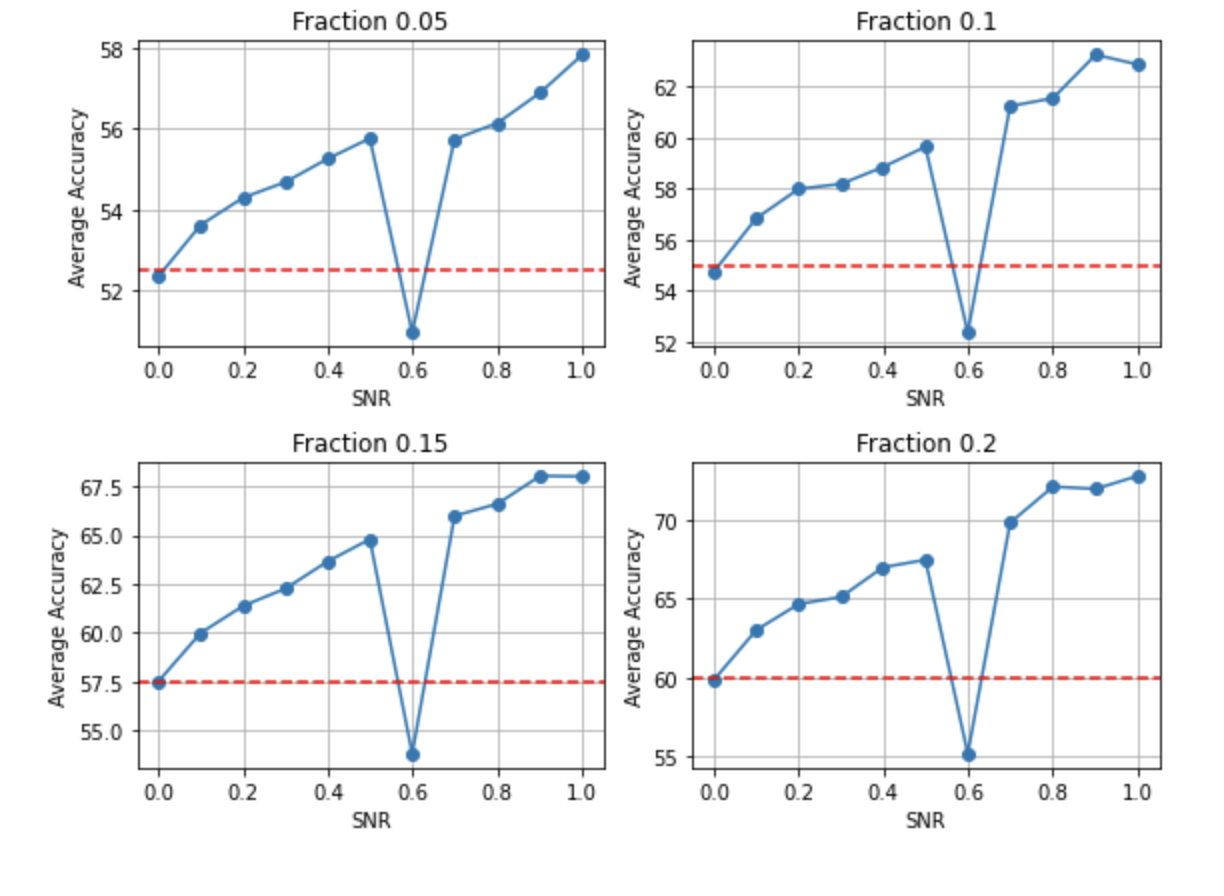
\includegraphics[width=1\linewidth]{Figures/Screenshot 2024-03-14 at 02.18.52.png}
    \caption{\textcolor{darkgray}{\small The spectrum in the complex plane of the non-backtracking matrix of a graph generated by the stochastic block mode. Here the eigenvector of the outlier eigenvalue u is correlated with the communities}}
    \label{fig:enter-label}
\end{figure}
\begin{figure}
    \centering
    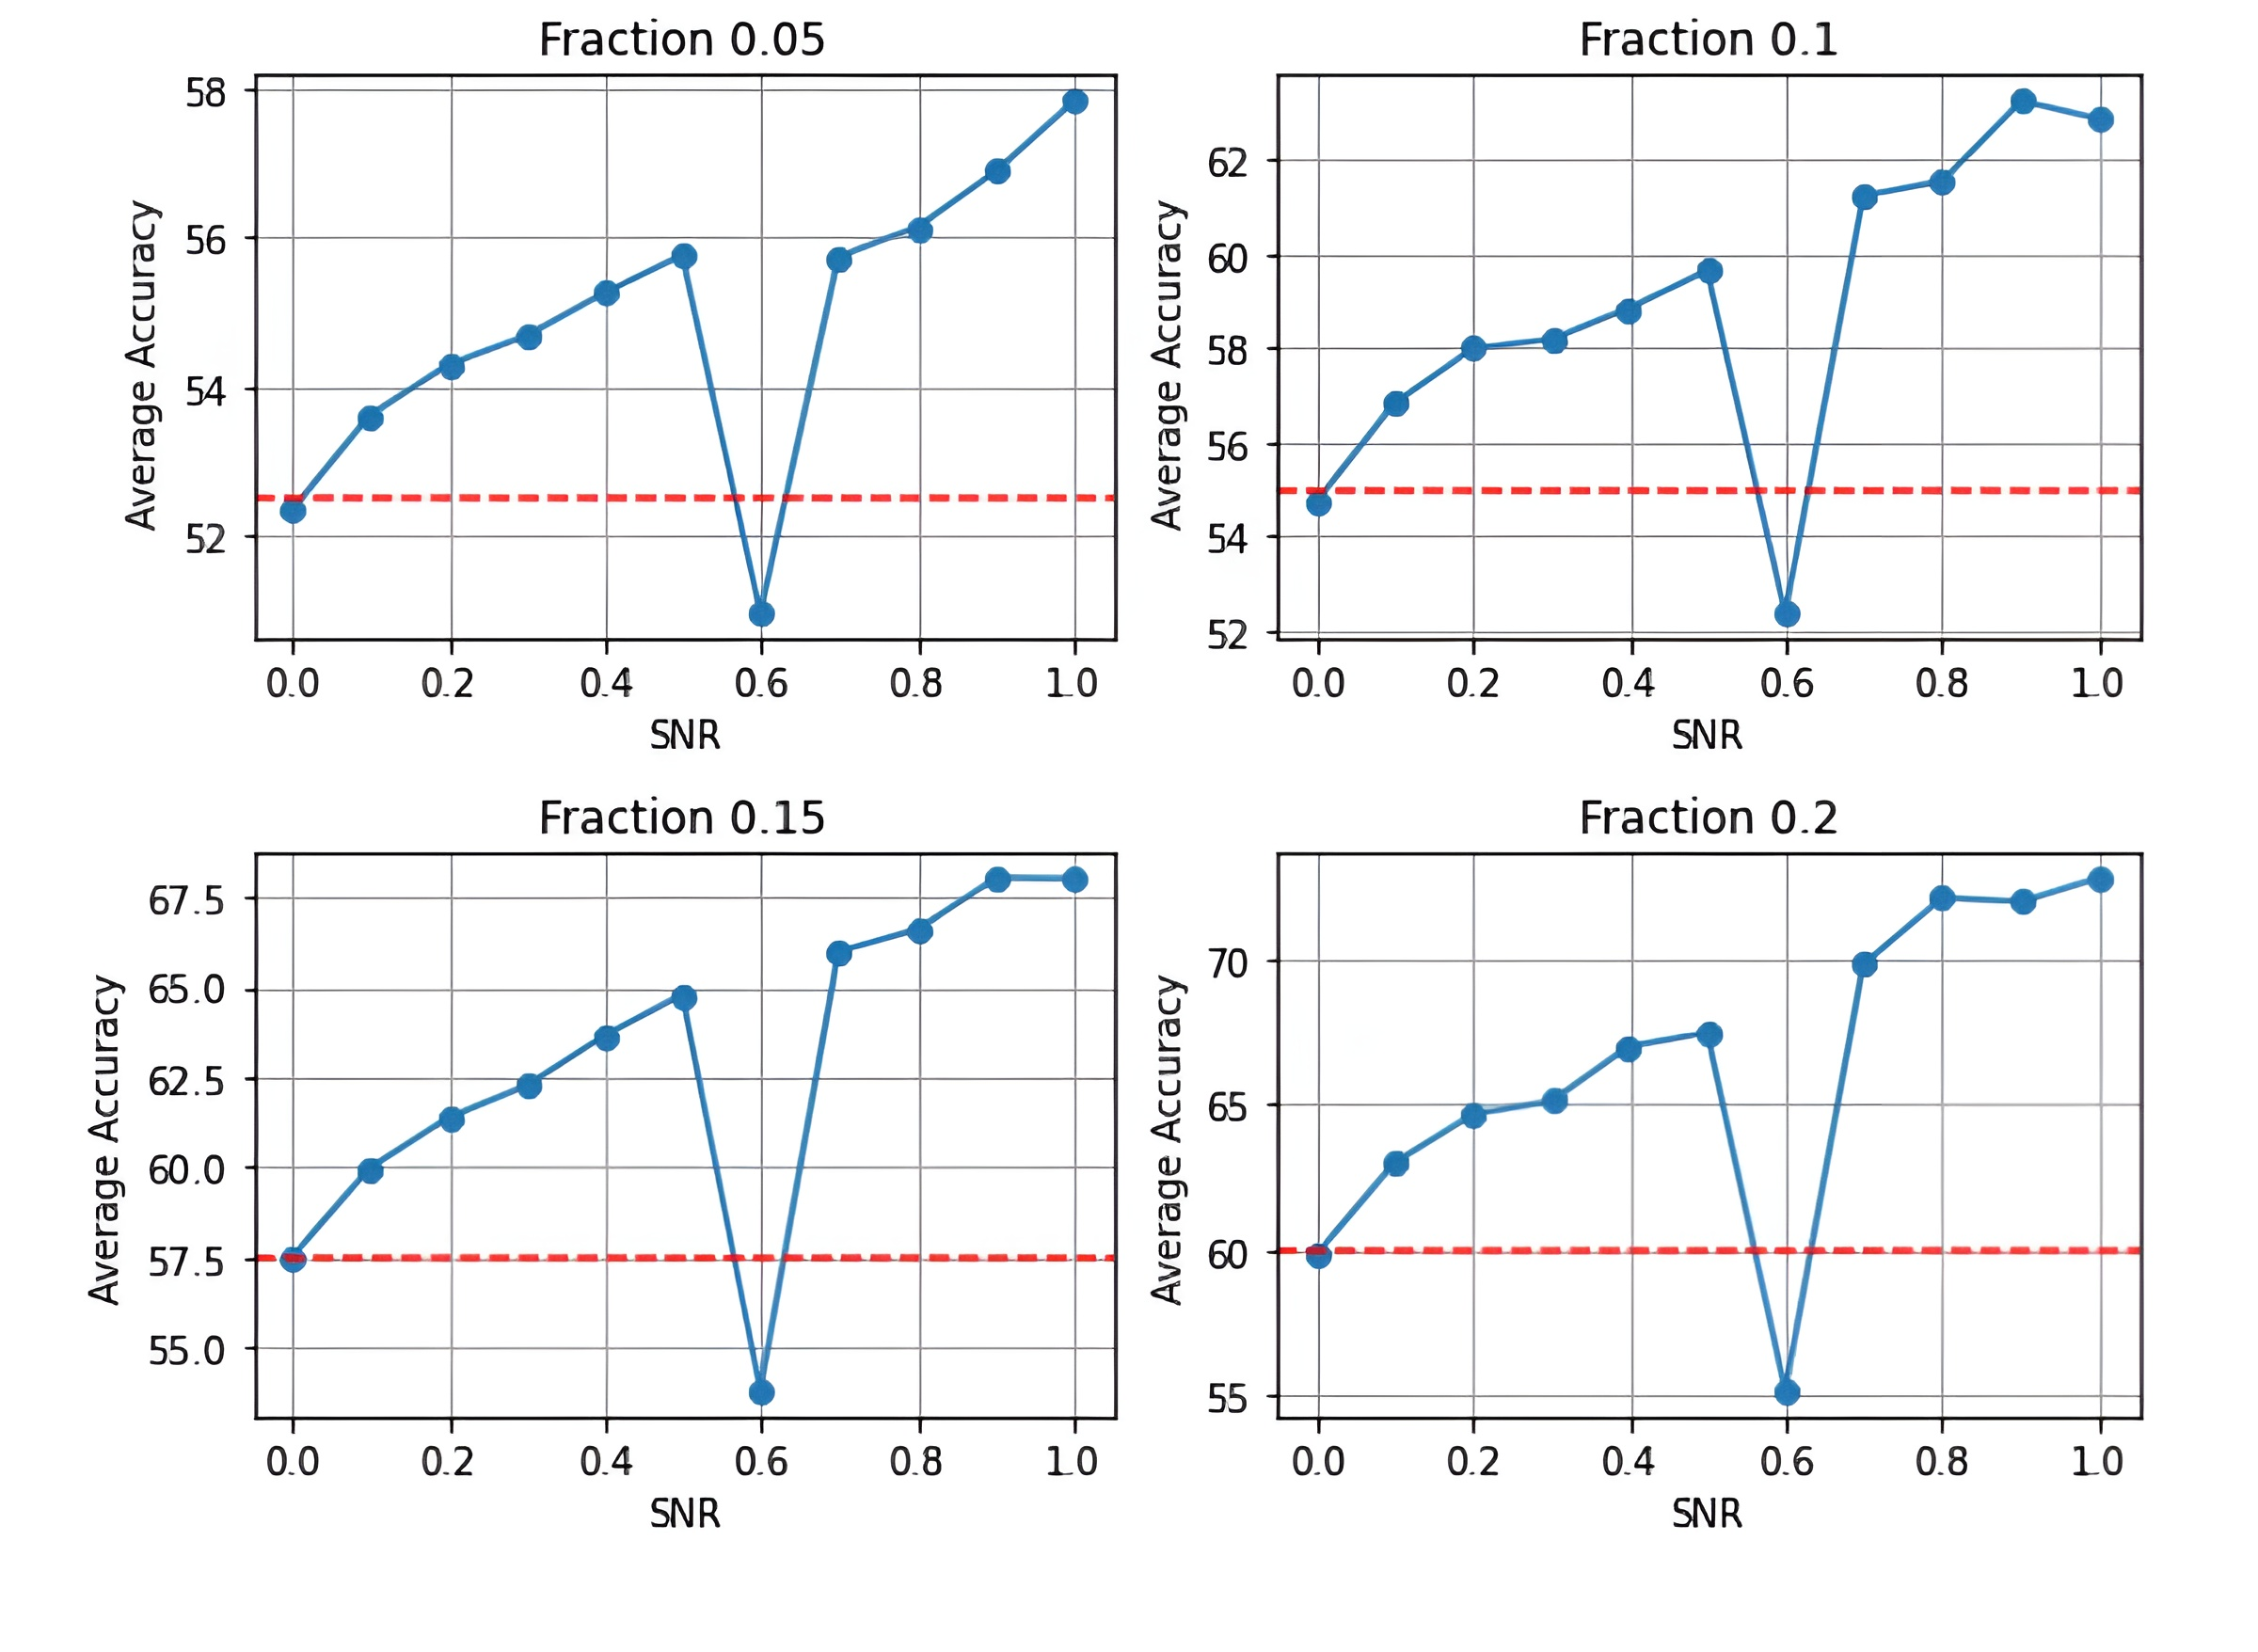
\includegraphics[width=1\linewidth]{Figures/Screenshot 2024-03-14 at 02.18.52.1.png}
    \caption{Enter Caption}
    \label{fig:enter-label}
\end{figure}
\begin{itemize}
    \item Objective 1
    \item Objective 2
    \item Objective 3
\end{itemize}